\section{Information-Theoretic Models}

\subsection{Interactive Proofs (IP)}

In this model, we have a prescribed "honest" deterministic prover algorithm $\mathcal{P}$ and a probabilistic polynomial-time verifier algorithm $\mathcal{V}$ (with internal randomness $r$). Given a common input $x$, the prover and verifier exchange messages and the verifier will output either \emph{accept} or \emph{reject} at the end of the protocol: \\

$$\text{out}(\mathcal{V}, x, r, \mathcal{P}) \in \{\text{accept},\text{reject}\}$$

\myspace

\begin{definition}[Interactive Proof System]
Let $(\mathcal{P}, \mathcal{V})$ be a $k$-message interactive proof system for a language $\mathcal{L} \subseteq \{0,1\}^n$. Then: \\

\textbf{Completeness:} For every $x \in \mathcal{L}$,
$$
\Pr_r[\text{out}(\mathcal{V}, x, r, \mathcal{P}) = 1] \ge 1 - \delta_c
$$

\textbf{Soundness:} For every $x \notin \mathcal{L}$ and any (possibly cheating) prover strategy $\mathcal{P}'$,
$$
\Pr_r[\text{out}(\mathcal{V}, x, r, \mathcal{P}') = 1] \le \delta_s
$$

Here, $\delta_c$ denotes the completeness error and  $\delta_s$ denotes the soundness error.  
\end{definition}

\begin{remark}
The system is considered valid if $\delta_c, \delta_s$ are sufficiently small.
\end{remark}

\myspace

\begin{definition}[Argument System] An \emph{argument system} is an interactive proof in which the soundness
condition is only required to hold against prover strategies that run in polynomial time. This is known as \emph{computational soundness}.
\end{definition} \\

\noindent This is in contrast to the soundness from the previous definition which can be referred to as \emph{statistical soundness} (or information-theoretic soundness). Through the use of cryptographic primitives, e.g., \emph{polynomial commitment schemes}, we can introduce such form of handicaps to the prover. This use of cryptography often allows argument systems to achieve additional desirable  properties, i.e. succinctness, non-interactivity, etc., that are unattainable for interactive proofs. \\

\begin{remark}
Additionally, the system may satisfy some knowledge properties described in Section 1.5.
\end{remark}

\myspace

\subsection*{Example: IP for SAT}

\subsubsection*{Problem Definition}

The satisfiability problem (SAT) asks whether a given boolean formula $\phi$ in conjunctive normal form (CNF) is satisfiable. Formally, let $\phi$ be a CNF formula over variables $x_1, \dots, x_n$ with disjunctive clauses $C_1, \dots, C_m$:
$$
\phi(x_1,\dots,x_n) = \bigwedge_{j=1}^m C_j
$$

\noindent Then language of satisfiable formulas is given by:
\[
\text{SAT} = \{\;\phi \mid \exists \, a \in \{0,1\}^n \;\; \text{s.t. } \phi(a)=1 \;\}
\]

\noindent In this setting, the common input is $\phi$ and the prover wishes to convince the verifier that $\phi \in \text{SAT}$.

\myspace

\begin{protocol}
\begin{enumerate}
  \item \textbf{Prover $\mathcal{P}$:} Sends a candidate assignment $a\in\{0,1\}^n$ to the verifier.
  \item \textbf{Verifier $\mathcal{V}$:} Samples $j \xleftarrow{\$} [m]$ uniformly at random and sends $j$ to $\mathcal{P}$.
  \item \textbf{Verifier $\mathcal{V}$:} Checks $C_j(a)=1$. If so, output \emph{accept}; otherwise, \emph{reject}.
\end{enumerate}
\end{protocol}

\paragraph{Completeness.}
If $\phi$ is satisfiable, then there exists $a^\star$ with $\phi(a^\star)=1$ so $C_j(a^\star)=1$ for all $j\in[m]$. \\
\noindent The honest prover sends $a^\star$ and the verifier accepts with probability $1$.

\paragraph{Soundness.}
Suppose $\phi$ is unsatisfiable. Then, for every assignment $a \in \{0,1\}^n$, there is at least one clause $C_j$ that is not satisfied, i.e., $C_j(a) = 0$. \\

\noindent Let:
\[
s(a) \;=\; \underbrace{\left|\{j \in [m] : C_j(a) = 1\}\right|}_{\text{number of clauses satisfied by } a} \;\le\; m-1
\]

\noindent Since $j$ is uniform in $[m]$, the probability that the verifier accepts a single round is:
\[
\Pr[\text{accept}] \;=\; \frac{s(a)}{m} \;\le\; 1-\frac{1}{m}
\]
By repeating the protocol independently for $k$ rounds, the soundness error decreases exponentially:
\[
\Pr[\text{verifier accepts all $k$ rounds}] \;\le\; \left(1-\frac{1}{m}\right)^k.
\]

\noindent Thus, by choosing $k$ appropriately, the soundness error can be made arbitrarily small. \\

\noindent \textit{\underline{Note}: This is an illustrative example. We will discuss performance considerations in future sections.}

\myspace

\begin{remark}
    This protocol does not yield negligible soundness error unless repeated many times but it illustrates how randomness allows the verifier to check global structure using only local queries.
\end{remark}

\subsection*{Example: The Sum-Check Protocol}

\subsubsection*{Problem Definition}

Suppose we are given a $v$-variate polynomial $g$ defined over a finite field $\mathbb{F}$. \\
The sum-check protocol allows a verifier to efficiently check claims of the following sum: 
$$
H := \sum_{x_1 \in \{0,1\}} \dots \sum_{x_n \in \{0,1\}} g(x_1, \dots, x_v),
$$ 

\begin{protocol}
\begin{enumerate}
  \item \textbf{Round 1:} \(\mathcal{P}\) sends the univariate polynomial:
  \[
    g_1(X_1) = \sum_{x_2,\dots,x_v \in \{0,1\}^{v-1}} g(X_1,x_2,\dots,x_v)
  \]
  \(\mathcal{V}\) checks that $g_1$ is a univariate polynomial of degree at most $\text{deg}_1(g)$, and that $H = g(0) + g(1)$. \\
  \(\mathcal{V}\) chooses a random element $r_1 \in \mathbb{F}$ and sends $r_1$ to $\mathcal{P}$.
  \item \textbf{Round \(i\) (\(2 \le i \le v\)):} \(\mathcal{P}\) sends the univariate polynomial:
  \[
    g_i(X_i) = \sum_{x_{i+1},\dots,x_v \in \{0,1\}^{v-i}} g(r_1, \dots, r_{i-1}, X_i, x_{i+1}, \dots, x_v)
  \]
   \(\mathcal{V}\) checks that $g_i$ is a univariate polynomial of degree at most $\text{deg}_i(g)$, and that $g_{i-1}(r_{i-1}) = g_i(0) + g_i(1)$. \(\mathcal{V}\) chooses a random element $r_i \in \mathbb{F}$ and sends $r_i$ to $\mathcal{P}$.
  \item \textbf{Final Check:} After round \(v\), \(\mathcal{V}\) evaluates \(g(r_1, \dots, r_v)\) directly and verifies consistency with \(g_v(r_v)\). \(\mathcal{V}\) outputs \emph{accept} if all checks pass.
\end{enumerate}
\end{protocol}

\myspace
\myspace

\noindent \textbf{Example:} Full Tree Illustrating The Sum-Check Protocol (where $v = 3$)

\myspace
\myspace

\noindent \resizebox{\textwidth}{!}{
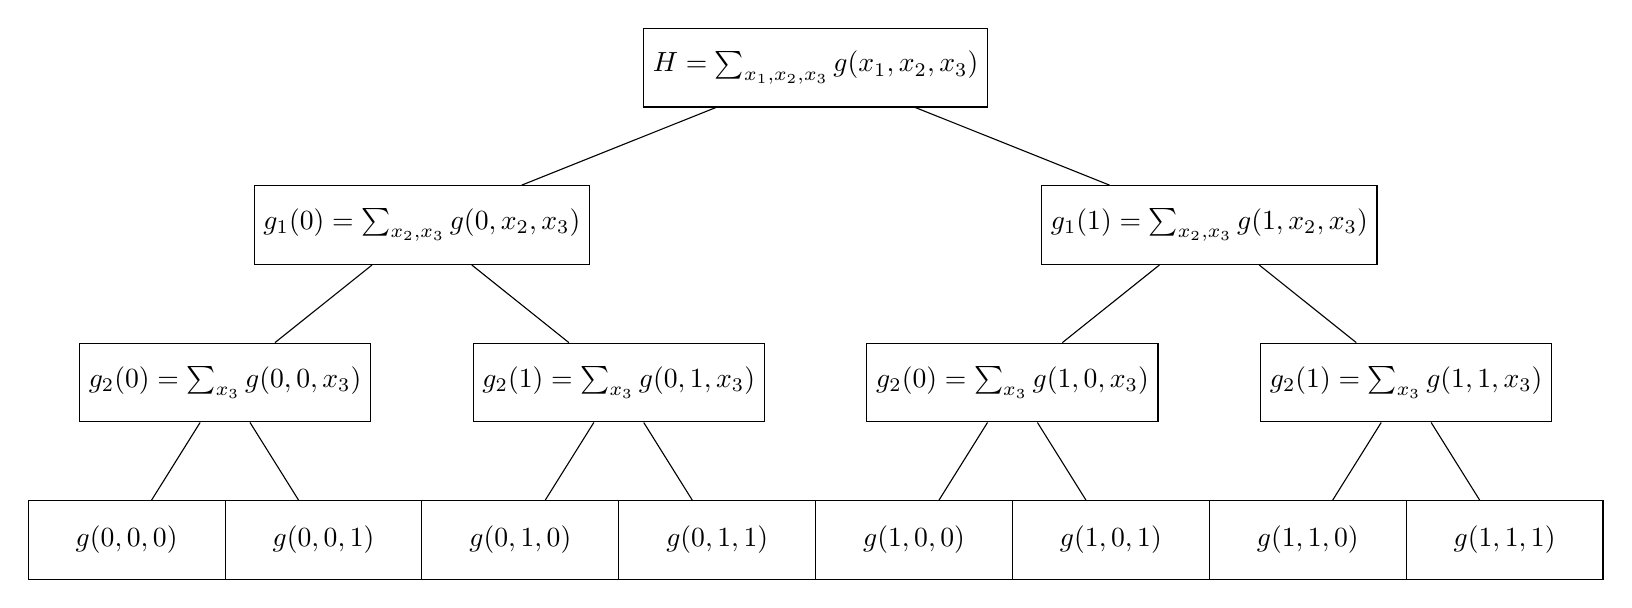
\begin{tikzpicture}[
  level distance=2cm,
  level 1/.style={sibling distance=10cm},
  level 2/.style={sibling distance=5cm},
  level 3/.style={sibling distance=2.5cm},
  every node/.style={draw, rectangle, minimum width=2.5cm, minimum height=1cm, align=center}
]

% Root node
\node {$H = \sum_{x_1,x_2,x_3} g(x_1,x_2,x_3)$}
  % Level 1
  child {node {$g_1(0) = \sum_{x_2,x_3} g(0,x_2,x_3)$}
    % Level 2
    child {node {$g_2(0) = \sum_{x_3} g(0,0,x_3)$}
      % Level 3
      child {node {$g(0,0,0)$}}
      child {node {$g(0,0,1)$}}
    }
    child {node {$g_2(1) = \sum_{x_3} g(0,1,x_3)$}
      child {node {$g(0,1,0)$}}
      child {node {$g(0,1,1)$}}
    }
  }
  child {node {$g_1(1) = \sum_{x_2,x_3} g(1,x_2,x_3)$}
    child {node {$g_2(0) = \sum_{x_3} g(1,0,x_3)$}
      child {node {$g(1,0,0)$}}
      child {node {$g(1,0,1)$}}
    }
    child {node {$g_2(1) = \sum_{x_3} g(1,1,x_3)$}
      child {node {$g(1,1,0)$}}
      child {node {$g(1,1,1)$}}
    }
  };
\end{tikzpicture}
}

\myspace
\myspace

\paragraph{Completeness.}
Similar argument to IP for SAT.

\myspace
\myspace
\hrule

\begin{theorem}[Schwartz--Zippel Lemma]
Let $\mathbb{F}$ be a finite field. Let $p \in \mathbb{F}[x_1,\dots,x_n]$ be a non-zero polynomial
of total degree $d \ge 0$. Choose $r=(r_1,\dots,r_n)$ uniformly at random from $\mathbb{F}^n$.
Then
\[
\Pr_{r\in \mathbb{F}^n}[\,p(r)=0\,] \;\le\; \frac{d}{|\mathbb{F}|}.
\]
\end{theorem}

\hrule
\myspace

\paragraph{Soundness.}
Suppose \(\mathcal{P}'\) sends a wrong polynomial \(g_i\) at some round \(i\). Let $g^*_i$ denote the correct polynomial at this round. Observe that $g_i - g^*_i$ is a non-zero polynomial of degree at most $\deg_i(g)$. The verifier chooses $r_i \in \mathbb{F}$ uniformly at random and continues only if $g_i(r_i) = g^*_i(r_i)$. \\

\noindent By Theorem 1.1, we know the following:
\[
\Pr[\,g_i(r_i) - g^*_i(r_i) =0\,] \;\le\; \frac{\deg_i(g)}{|\mathbb{F}|}.
\]
If this equality check does not hold, then the verifier rejects immediately. Thus, the protocol continues with a wrong polynomial in round $i$ with probability at most $\deg_i(g)/|\mathbb{F}|$. \\

\noindent Applying a union bound over all $v$ rounds, the overall soundness error is bounded by the following:
\[
\delta_{s} \;\le\; \sum_{i=1}^v \frac{\deg_i(g)}{|\mathbb{F}|}.
\]
In particular, if $d=\max_i \deg_i(g)$, then:
\[
\delta_{s} \;\le\; \frac{v \cdot d}{|\mathbb{F}|}.
\]
Thus, by choosing $\mathbb{F}$ to be sufficiently large, the soundness error can be made arbitrarily small. \\


\subsection{Multi-prover Interactive Proofs (MIP)}

We can generalize interactive proofs by introducing multiple provers. These provers may coordinate on a joint strategy beforehand but are not able to communicate during the protocol. \\

\noindent Let $k \ge 2$. A \emph{$k$-prover interactive proof system} for a language $\mathcal{L} \subseteq \{0,1\}^n$ involves $k+1$ parties: a probabilistic polynomial-time verifier $\mathcal{V}$ and $k$ provers $\mathcal{P}_1, \dots, \mathcal{P}_k$.  Given a common input $x$, the provers and verifier exchange messages and the verifier will output either \emph{accept} or \emph{reject} at the end of the protocol: \\

$$\text{out}(\mathcal{V}, x, r, \mathcal{P}_1, \dots, \mathcal{P}_k) \in \{\text{accept},\text{reject}\}$$

\myspace

\begin{definition}[Multi-Prover Interactive Proof System] Let $(\mathcal{P}_1, \dots, \mathcal{P}_k, \mathcal{V})$ be a k-party interactive proof system for a language $\mathcal{L} \subseteq \{0,1\}^n$. Then:

\begin{itemize}
    \item \textbf{Completeness:} There exists a tuple of prover strategies $(\mathcal{P}_1, \dots, \mathcal{P}_k)$ such that for every $x \in \mathcal{L}$,
    \[
    \Pr_r[\text{out}(\mathcal{V}, x, r, \mathcal{P}_1, \dots, \mathcal{P}_k) = \text{accept}] \ge 1 - \delta_c.
    \]
    
    \item \textbf{Soundness:} For every $x \notin \mathcal{L}$ and for every tuple of prover strategies $(\mathcal{P}'_1, \dots, \mathcal{P}'_k)$,
    \[
    \Pr_r[\text{out}(\mathcal{V}, x, r, \mathcal{P}'_1, \dots, \mathcal{P}'_k) = \text{accept}] \le \delta_s.
    \]
\end{itemize}

Here, $\delta_c$ denotes the completeness error and  $\delta_s$ denotes the soundness error.  
\end{definition}

\begin{remark}
The system is considered valid if $\delta_c, \delta_s$ are sufficiently small.
\end{remark} \\

\begin{remark}
The primary advantage of multiple provers is non-adaptivity, i.e., preventing adaptive cheating strategies.
\end{remark}

\subsection*{Example: MIP for SAT}

\subsubsection*{Problem Definition}

Let $\phi$ be a 3-CNF (each clause contains exactly 3 literals) formula over variables $x_1,\dots,x_n$ with clauses $C_1,\dots,C_m$. Again, the common input is $\phi$, and the prover wishes to convince the verifier that $\phi \in \text{SAT}$.

\myspace

\begin{protocol}
\begin{enumerate}
  \item \textbf{Verifier $\mathcal{V}$:} Sample a clause index $j \xleftarrow{\$} [m]$ uniformly at random and a position $t \xleftarrow{\$} \{1,2,3\}$ uniformly at random. Let the $t$-th literal in $C_j$ be $\ell_{j,t}$ over variable $x_{i_{j,t}}$ (possibly negated).
  
  \item \textbf{Queries:}
  \begin{itemize}
    \item Send $j$ to $\mathcal{P}_1$ and request the three bits $(b_{j,1},b_{j,2},b_{j,3}) \in \{0,1\}^3$ giving purported values of the underlying variables of $C_j$ (in clause order).
    \item Send $(j,t)$ (or equivalently the variable index $i_{j,t}$) to $\mathcal{P}_2$ and request a single bit $c_{j,t}\in\{0,1\}$ giving the purported value of $x_{i_{j,t}}$.
  \end{itemize}
  
  \item \textbf{Checks:}
  \begin{itemize}
    \item \emph{Clause check:} Using $(b_{j,1},b_{j,2},b_{j,3})$, evaluate $C_j$; require $C_j(b_{j,1},b_{j,2},b_{j,3})=1$.
    \item \emph{Consistency check:} Require that $c_{j,t}$ equals the $t$-th component $b_{j,t}$.
  \end{itemize}
  
  \item \textbf{Decision:} Accept iff both checks pass.
\end{enumerate}
\end{protocol}

\paragraph{Completeness.}
If $\phi$ is satisfiable, fix a satisfying assignment $a^\star\in\{0,1\}^n$. The honest strategy is:
\[
\mathcal{P}_1(j)\;=\;(a^\star_{i_{j,1}},a^\star_{i_{j,2}},a^\star_{i_{j,3}}),\qquad
\mathcal{P}_2(j,t)\;=\;a^\star_{i_{j,t}}.
\]
Then $C_j$ is satisfied and the answers are consistent for all $(j,t)$, so $\mathcal{V}$ accepts with probability $1$.

\paragraph{Soundness.}
Suppose $\phi$ is unsatisfiable. Consider arbitrary (possibly cheating) strategies for $\mathcal{P}_1,\mathcal{P}_2$. Define a \emph{derived global assignment} $\tilde{a}\in\{0,1\}^n$ as follows: for each variable $x_i$, let $\tilde{a}_i$ be the bit that $\mathcal{P}_2$ would most commonly answer when asked for $x_i$ (break ties arbitrarily). Since $\phi$ is unsatisfiable, $\tilde{a}$ falsifies at least one clause; let $\mathcal{B}\subseteq [m]$ be the set of clauses falsified by $\tilde{a}$, so $\mathcal{B}\neq\emptyset$.

Fix any $j\in\mathcal{B}$. For clause $C_j$, one of the following must happen:
\begin{enumerate}
  \item \textbf{(Clause failure)} $\mathcal{P}_1$'s triple $(b_{j,1},b_{j,2},b_{j,3})$ fails to satisfy $C_j$. Then the verifier rejects regardless of $t$.
  \item \textbf{(Inconsistency)} $\mathcal{P}_1$ outputs a triple that \emph{does} satisfy $C_j$. Since $C_j$ is false under $\tilde{a}$, this triple must disagree with $\tilde{a}$ on at least one of the three variables of $C_j$. When the verifier’s random $t\in\{1,2,3\}$ hits any position where $b_{j,t}\neq \tilde{a}_{i_{j,t}}$, the consistency check tends to fail because $\mathcal{P}_2$ answers (with high bias) according to $\tilde{a}_{i_{j,t}}$. In particular, conditioned on clause $j$, the probability (over $t$) of catching a disagreement is at least $1/3$.
\end{enumerate}
Therefore, when $j$ is chosen uniformly from $[m]$ and $t$ uniformly from $\{1,2,3\}$, the verifier rejects with probability at least
\[
\Pr[j\in\mathcal{B}]\cdot \frac{1}{3} \;\ge\; \frac{1}{m}\cdot \frac{1}{3}\;=\;\frac{1}{3m},
\]
so the acceptance probability is at most $1-\frac{1}{3m}$. By independent parallel repetition (running the one-round protocol $k$ times and accepting only if all copies accept), the soundness error drops exponentially:
\[
\Pr[\text{accept all }k\text{ copies}] \;\le\; \left(1-\frac{1}{3m}\right)^k.
\]

\noindent \textit{\underline{Note}: This is an illustrative example. We will discuss performance considerations in future sections.} \\

\begin{remark}
This is the standard “oracularization” of an NP witness: $\mathcal{P}_1$ pretends to be a local view of the assignment on a random clause; $\mathcal{P}_2$ pretends to be a consistent oracle for single variables. The second prover enforces non-adaptivity/consistency, which is what you cannot get in the single-prover version without cryptographic tools. Two provers, one round already suffices for the usual MIP power phenomena (and is the canonical gateway to PCP).
\end{remark} 


\subsection{Probabilistically Checkable Proofs (PCP)}

In a PCP setting, the prover writes down a long proof string $\pi \in \{0,1\}^\ell$, and the verifier is allowed only \emph{oracle access} to $\pi$ (i.e., it may query a few positions). The verifier uses randomness to decide which positions of $\pi$ to read, and must decide whether to accept or reject based on those few symbols. \\

\noindent In MIP, if a prover is asked multiple questions (multiple rounds), then the prover can behave adaptively. This adaptivity is potentially bad for soundness since the ability to behave adaptively makes it harder to "pin down" the prover(s) in a lie. PCP mitigates this (although at the cost of efficiency). \\

\noindent A \emph{probabilistically checkable proof system (PCP)} for a language $\mathcal{L} \subseteq \{0,1\}^n$ consists of a probabilistic polynomial-time verifier $\mathcal{V}$ that is given access to a common input $x$ and \emph{oracle access} to a proof string $\pi \in \Sigma^\ell$ (where $\Sigma$ is the proof alphabet and $\ell$ is the length of the proof). 

\begin{definition}[Probabilistically Checkable Proof System]
Let $\mathcal{V}^{\pi}$ be a probabilistically checkable proof system for a language $\mathcal{L} \subseteq \{0,1\}^n$. Then:

\begin{itemize}
    \item \textbf{Completeness:} For every $x \in \mathcal{L}$, there exists a proof string $\pi \in \Sigma^\ell$ such that
    \[
    \Pr[\mathcal{V}^\pi(x) = \text{accept}] \ge 1 - \delta_c
    \]
    
    \item \textbf{Soundness:} For every $x \notin \mathcal{L}$ and every proof string $\pi \in \Sigma^\ell$,
    \[
    \Pr[\mathcal{V}^\pi(x) = \text{accept}] \le \delta_s
    \]
\end{itemize}

Here, $\delta_c$ denotes the completeness error and  $\delta_s$ denotes the soundness error.  
\end{definition}

\begin{remark}
The system is considered valid if $\delta_c, \delta_s$ are sufficiently small.
\end{remark} 

\subsection*{Example: PCP for SAT}

\subsubsection*{Problem Definition}

Same as above.


\myspace

\subsubsection*{Proof Generation}

Suppose $\phi$ is satisfiable and let $a^\star \in \{0,1\}^n$ be a satisfying assignment. The prover constructs a proof string $\pi$ that encodes $a^\star$ redundantly so that local consistency checks are possible. A canonical choice is to encode the \emph{truth table of the assignment as a linear error-correcting code} (e.g., Hadamard or Reed–Muller code).

Intuitively:
- Each variable assignment is spread across many positions of $\pi$.  
- Local queries to $\pi$ allow the verifier to check both \emph{consistency} (different parts of the proof agree on the same variable) and \emph{clause satisfaction}.  

\myspace

\begin{protocol}
\begin{enumerate}
  \item \textbf{Verifier $\mathcal{V}$:} Pick a random clause index $j \xleftarrow{\$}[m]$.
  
  \item \textbf{Verifier $\mathcal{V}$:} Query $\pi$ at a small number of locations sufficient to decode the purported values of the three variables in clause $C_j$. Denote these values $(b_{j,1},b_{j,2},b_{j,3})$.
  
  \item \textbf{Verifier $\mathcal{V}$:} Check that the tuple $(b_{j,1},b_{j,2},b_{j,3})$ is consistent with the error-correcting code used for $\pi$ (this enforces that all queried bits come from some global assignment).
  
  \item \textbf{Verifier $\mathcal{V}$:} Evaluate $C_j(b_{j,1},b_{j,2},b_{j,3})$.  
  Accept if it evaluates to $1$ and the consistency check passes; otherwise reject.
\end{enumerate}
\end{protocol}

\paragraph{Completeness.}
If $\phi \in \text{SAT}$ with satisfying assignment $a^\star$, the honest prover encodes $a^\star$ into $\pi$ using the agreed-upon code. Then:
- Every local view of $\pi$ is consistent with some assignment.  
- For every clause $C_j$, the tuple $(b_{j,1},b_{j,2},b_{j,3})$ derived from $\pi$ makes $C_j$ true.  
Thus, the verifier always accepts.

\paragraph{Soundness.}
Suppose $\phi \notin \text{SAT}$. Then no assignment satisfies all clauses. Any proof string $\pi$ necessarily encodes information corresponding (at best) to some assignment $\tilde{a}$. Since $\tilde{a}$ falsifies at least one clause, there exists some $j \in [m]$ for which $C_j(\tilde{a})=0$.  

When the verifier samples this clause and decodes the corresponding tuple from $\pi$, one of two things happens:
\begin{itemize}
  \item The decoded triple fails the clause check $\implies$ verifier rejects.  
  \item The decoded triple passes the clause check but is inconsistent with the purported codeword $\implies$ verifier rejects in the consistency check.  
\end{itemize}
Thus, with non-negligible probability (at least $1/m$), the verifier rejects. \\

By repeating with fresh randomness, the soundness error decreases exponentially.

\myspace

\begin{remark}
This toy construction illustrates the PCP idea:  
\begin{enumerate}
  \item The prover commits to a long, redundant proof string $\pi$.  
  \item The verifier uses only a few random queries to $\pi$ to check both consistency and clause satisfaction.  
\end{enumerate}
In practice, real PCP constructions (e.g., using low-degree tests and robust codes) achieve stronger guarantees: \emph{constant query complexity} and \emph{constant soundness error}, independent of $n$ or $m$.
\end{remark}

\subsubsection*{Linear PCP}

\noindent A linear PCP is a special case of a PCP where the proof $\pi$ is interpreted as a vector over a finite field $\mathbb{F}$ and the verifier’s queries are linear functionals of the proof. This structure enables algebraic manipulation and is a building block for many efficient cryptographic protocols.

\begin{definition}[Linear PCP]
A \emph{linear probabilistically checkable proof} for a language $\mathcal{L} \subseteq \{0,1\}^n$ consists of a proof vector $\pi \in \mathbb{F}^\ell$ and a verifier $\mathcal{V}$ such that:
\begin{itemize}
    \item The verifier chooses a random linear query $q \in \mathbb{F}^\ell$ and computes the inner product $\langle q, \pi \rangle$.
    \item \textbf{Completeness:} If $x \in \mathcal{L}$, the honest proof $\pi$ satisfies $\mathcal{V}$’s checks with probability $\ge 1-\delta_c$.
    \item \textbf{Soundness:} If $x \notin \mathcal{L}$, any $\pi$ passes the verifier’s checks with probability $\le \delta_s$.
\end{itemize}
\end{definition}

\begin{remark}[Intuition]
Linear PCPs are useful because linear operations commute with many algebraic encodings (like error-correcting codes).  
The verifier can check consistency and correctness of the proof using only a few inner products, enabling succinct, locally checkable proofs.
\end{remark}


\subsection{Interactive Oracle Proofs (IOP)}

An Interactive Oracle Proof is a unifying abstraction that generalizes both interactive proofs and PCPs. As in an IP, the verifier and prover exchange messages in multiple rounds. As in a PCP, the verifier can access messages from the prover non-adaptively via \emph{oracle queries} rather than reading them in full. \\

Formally, an IOP proceeds in $t$ rounds. In each round $i$:
\begin{enumerate}
    \item The verifier $\mathcal{V}$ sends a message $m_i$.
    \item The prover $\mathcal{P}$ replies with a string $\pi_i \in \Sigma^{\ell_i}$ (which is treated as an oracle).
    \item The verifier may query at most $q_i$ positions of $\pi_i$, (with queries chosen adaptively based on answers received so far in the round).
\end{enumerate}

At the end of the protocol, the verifier outputs either \emph{accept} or \emph{reject}.

\begin{definition}[Interactive Oracle Proof System]
Let $(\mathcal{P}, \mathcal{V})$ be a \emph{interactive oracle proof system} for a language. Then:
\begin{itemize}
    \item \textbf{Completeness:} For every $x \in \mathcal{L}$,
    \[
    \Pr_r[\mathcal{V}^{\pi_1,\dots,\pi_t}(x) = \text{accept}] \ge 1 - \delta_c,
    \]
    where $\pi_1,\dots,\pi_t$ are the oracles provided by the honest prover strategy $\mathcal{P}$.
    \item \textbf{Soundness:} For every $x \notin \mathcal{L}$ and every (possibly cheating) prover strategy $\mathcal{P}'$ producing oracle strings $\pi_1',\dots,\pi_t'$,
    \[
    \Pr_r[\mathcal{V}^{\pi_1',\dots,\pi_t'}(x) = \text{accept}] \le \delta_s.
    \]
\end{itemize}
Here, $\delta_c$ denotes the completeness error and  $\delta_s$ denotes the soundness error.  
\end{definition}

\begin{remark}
The system is considered valid if $\delta_c, \delta_s$ are sufficiently small.
\end{remark} 

Observe that the IOP model reduces to an IP if the verifier reads each oracle in full and to a PCP if there is only one round and the verifier sends no messages.

\subsection*{IOP for SAT}

\subsubsection*{Problem Definition}

Same SAT setup as before: input $\phi$ is a CNF formula with clauses $C_1,\dots,C_m$, and the prover wishes to convince the verifier that $\phi \in \text{SAT}$. 

\myspace

\begin{protocol}
\begin{enumerate}
  \item \textbf{Round 1:}  
  \(\mathcal{P}\) sends $\pi_1$, which is an error-correcting encoding of a candidate assignment $a \in \{0,1\}^n$.  
  \(\mathcal{V}\) commits to a random clause index $j \in [m]$, but does not reveal it yet.

  \item \textbf{Round 2:}  
  \(\mathcal{P}\) sends $\pi_2$, designed so that the verifier can query the three variables appearing in clause $C_j$ using only a few locations of $\pi_2$.  

  \item \textbf{Verifier Queries:}  
  \(\mathcal{V}\) makes a small number of queries to $\pi_1$ and $\pi_2$:  
  \begin{itemize}
    \item From $\pi_1$: check that queried symbols are consistent with a valid codeword (linear consistency check).  
    \item From $\pi_2$: decode the tuple $(b_{j,1},b_{j,2},b_{j,3})$ corresponding to the three literals in $C_j$.  
  \end{itemize}

  \item \textbf{Check and Decision:}  
  \(\mathcal{V}\) verifies that the tuple from $\pi_2$ is consistent with $\pi_1$, and that $C_j(b_{j,1},b_{j,2},b_{j,3})=1$.  
  Accept if both checks pass; otherwise reject.
\end{enumerate}
\end{protocol}

\paragraph{Completeness.}
If $\phi$ is satisfiable with assignment $a^\star$, the honest prover encodes $a^\star$ into both $\pi_1$ and $\pi_2$.  
- Consistency queries succeed since both are encodings of the same assignment.  
- Clause queries succeed since $a^\star$ satisfies every clause.  
Thus the verifier always accepts.

\paragraph{Soundness.}
If $\phi$ is unsatisfiable, then for any encoding $\pi_1,\pi_2$, there exists a clause $C_j$ that is falsified by the derived assignment. With probability at least $1/m$, the verifier selects such a clause.  
\begin{itemize}
  \item If $\pi_2$ encodes values that falsify $C_j$, the clause check fails.  
  \item If $\pi_2$ encodes values that make $C_j$ true but are inconsistent with $\pi_1$, the consistency check fails.  
\end{itemize}
Hence the verifier rejects with noticeable probability. By independent repetition, the soundness error decreases exponentially:
\[
\Pr[\text{accept all $k$ repetitions}] \;\le\; \left(1-\tfrac{1}{m}\right)^k.
\]

\subsection{Linear IOP}

\noindent A linear IOP generalizes linear PCPs to multiple rounds with interactive messages. The verifier can still query the prover’s messages as linear functions over a finite field. This allows for interaction while preserving algebraic structure.

\begin{definition}[Linear Interactive Oracle Proof]
A \emph{linear IOP} for a language $\mathcal{L} \subseteq \{0,1\}^n$ consists of:
\begin{itemize}
    \item A multi-round interaction between a prover $\mathcal{P}$ and verifier $\mathcal{V}$.
    \item In each round $i$, the prover sends an oracle string $\pi_i \in \mathbb{F}^{\ell_i}$.
    \item The verifier makes a bounded number of \emph{linear queries} $q_i \in \mathbb{F}^{\ell_i}$ and checks $\langle q_i, \pi_i \rangle$.
    \item \textbf{Completeness:} If $x \in \mathcal{L}$, the honest prover ensures $\mathcal{V}$ accepts with probability $\ge 1-\delta_c$.
    \item \textbf{Soundness:} If $x \notin \mathcal{L}$, no prover strategy passes with probability more than $\delta_s$.
\end{itemize}
\end{definition}

\begin{remark}[Intuition]
Linear IOPs combine the algebraic structure of linear PCPs with interaction.  
This allows the verifier to check complex claims efficiently over multiple rounds while maintaining local linear checks.  
Many modern SNARK/STARK constructions are based on linear IOP frameworks.
\end{remark}

\subsection{Knowledge Properties}

Beyond completeness and soundness, cryptographic applications often require stronger guarantees
about what the prover ``knows'' and what the verifier ``learns.'' Two fundamental refinements are
\emph{knowledge soundness} (also called \emph{proof of knowledge}) and \emph{zero-knowledge}.

\myspace

\noindent We first formalize what the verifier ``sees'' during an execution.

\begin{definition}[View]
Let $(\mathcal{P}, \mathcal{V})$ be an interactive proof. Let $x$ be a common input. The \emph{view} of the verifier $\mathcal{V}$ on the input $x$ in an interaction with the prover $\mathcal{P}$ consists of the transcript (sequence of messages exchanged) and its internal randomness $r$, and internal state. We denote this distribution by:
$$
\mathrm{view}_{\mathcal{V}}(\langle \mathcal{P},\mathcal{V}\rangle(x))
$$
\end{definition}

\begin{definition}[Indistinguishability] Some notions of indistinguishability:
\begin{itemize}
\item \emph{Perfect Indistinguishability}: $D_1 = D_2$.
 \item \emph{Statistical Indistinguishability}: for all $n$,
  \[
  \Delta(D_1(n),D_2(n)) = \tfrac{1}{2} \sum_{z} \big| \Pr[D_1(n)=z] - \Pr[D_2(n)=z] \big|
  \leq \text{negl}(n).
  \]

  \item \emph{Computational Indistinguishability}: for every probabilistic polynomial-time distinguisher $\mathcal{D}$ there exists a negligible function $\mu(\cdot)$ such that for all $n$,
  \[
  \big| \Pr[\mathcal{D}(D_1(n))=1] - \Pr[\mathcal{D}(D_2(n))=1] \big| \leq \mu(n).
  \]
\end{itemize}
\end{definition}

\begin{definition}[Knowledge Extractor]
Let $(\mathcal{P},\mathcal{V})$ be an interactive proof system for a relation $R$.
A \emph{knowledge extractor} $\mathcal{K}$ is a probabilistic polynomial-time algorithm
with (black-box) oracle access to a possibly malicious prover $\mathcal{P}^*$,
such that for any input $x \in L$ and any $\mathcal{P}^*$ that convinces $\mathcal{V}$ to accept $x$ 
with non-negligible probability $\varepsilon(n)$, the extractor $\mathcal{K}^{\mathcal{P}^*}(x)$
outputs a witness $w$ satisfying $(x,w)\in R$ with probability at least $\varepsilon(n) - \text{negl}(n)$,
where $\text{negl}(n)$ is a negligible function in the security parameter $n$.
\end{definition}

\begin{remark}[Intuition]
Intuitively, the extractor tries to ``observe'' the prover's strategy to obtain enough information 
to reconstruct a valid witness. In many protocols, this is accomplished via \emph{rewinding}:
the extractor runs the prover multiple times with different verifier randomness and uses the
differences between accepting transcripts to efficiently compute a witness.
This technique captures the idea that a prover cannot convince the verifier without actually ``knowing'' a valid witness.
\end{remark}

\begin{definition}[Simulator]
Let $(\mathcal{P}, \mathcal{V})$ be an interactive proof system for a language $L$.
A \emph{simulator} $\mathcal{S}$ is a probabilistic polynomial-time algorithm such that
for every input $x \in L$, the distribution
$
\mathcal{S}(x)
$
is (perfectly / statistically / computationally) indistinguishable from
the view of the verifier when interacting with the honest prover:
\[
\mathcal{S}(x) \approx \mathrm{view}_{\mathcal{V}}(\langle \mathcal{P}, \mathcal{V} \rangle(x)).
\]

\noindent Intuitively, $\mathcal{S}$ generates what the verifier would see in the real protocol
\emph{without any interaction with the prover}, thus capturing the idea that the protocol leaks no additional information.
\end{definition}


\myspace

\noindent Ordinary soundness only guarantees that if the verifier accepts, the statement is true.
It does not imply that the prover ``knows'' a witness. Knowledge soundness strengthens this by
requiring that any prover that convinces the verifier can be used to extract a valid witness.

\begin{definition}[Proof of Knowledge / Knowledge Soundness]
An interactive proof system $(\mathcal{P},\mathcal{V})$ for a relation $R$ is a 
\emph{proof of knowledge} if there exists a probabilistic polynomial-time algorithm 
$\mathcal{K}$ (the \emph{knowledge extractor}) such that for every (possibly malicious) prover 
$\mathcal{P}^*$ and input $x$, if
\[
\Pr[\langle \mathcal{P}^*(x), \mathcal{V}(x)\rangle = \text{accept}] \geq \varepsilon,
\]
then $\mathcal{K}^{\mathcal{P}^*}(x)$ outputs a witness $w$ such that $(x,w)\in R$
with probability at least $\varepsilon - \text{negl}(n)$.
\end{definition}

\begin{remark}
The extractor $\mathcal{K}$ is given black-box access to the prover $\mathcal{P}^*$ and may use
techniques such as \emph{rewinding} to obtain multiple executions of the interaction.
Intuitively: if a prover can convince the verifier, then it must ``know'' a valid witness,
because the extractor can efficiently obtain one.
\end{remark}

\myspace

\noindent Zero-knowledge ensures that the verifier learns nothing beyond the validity of the statement.
This is formalized by the existence of a simulator that can reproduce the verifier's view
without interacting with the prover.

\begin{definition}[Zero-Knowledge]
An interactive proof system $(\mathcal{P},\mathcal{V})$ for a language $L$ is
\emph{zero-knowledge} if for every probabilistic polynomial-time verifier
$\mathcal{V}^*$ there exists a simulator $\mathcal{S}$ such that for all $x \in L$,
\[
\mathrm{view}_{\mathcal{V}^*}(\langle \mathcal{P},\mathcal{V}^*\rangle(x))
\approx \mathcal{S}(x),
\]
where $\approx$ denotes either perfect, statistical, or computational indistinguishability.
\end{definition}

\myspace

\noindent Combining both notions yields zero-knowledge proofs of knowledge (ZKPoKs), where the prover
convinces the verifier of a statement, while simultaneously ensuring the verifier learns nothing
beyond validity, and the prover must ``know'' a witness.

\begin{definition}[Zero-Knowledge Proof of Knowledge]
An interactive proof system $(\mathcal{P},\mathcal{V})$ for a relation $R$ is a 
\emph{zero-knowledge proof of knowledge} if it is both zero-knowledge and a proof of knowledge.
\end{definition}

\begin{remark}
ZKPoKs are the foundation of many modern cryptographic protocols, including succinct
arguments (SNARGs) and their efficient variants (SNARKs, STARKs).
\end{remark}

% \subsection{Complexity Results}

% \subsubsection*{IP = PSPACE}
% \subsubsection*{MIP = NEXP}
% \subsubsection*{MIP $\leftrightarrow$ PCP}
% \subsubsection*{PCP Theorem}